
\chapter{Entwurf}
\section{Systementwurf}
\subsection{Generelles Data Fetching} \label{data-fetching}
Dieses Abschnitt baut auf das Kapitel \ref{oauth2-strat} auf.
\begin{figure}[!ht]
  \centering
  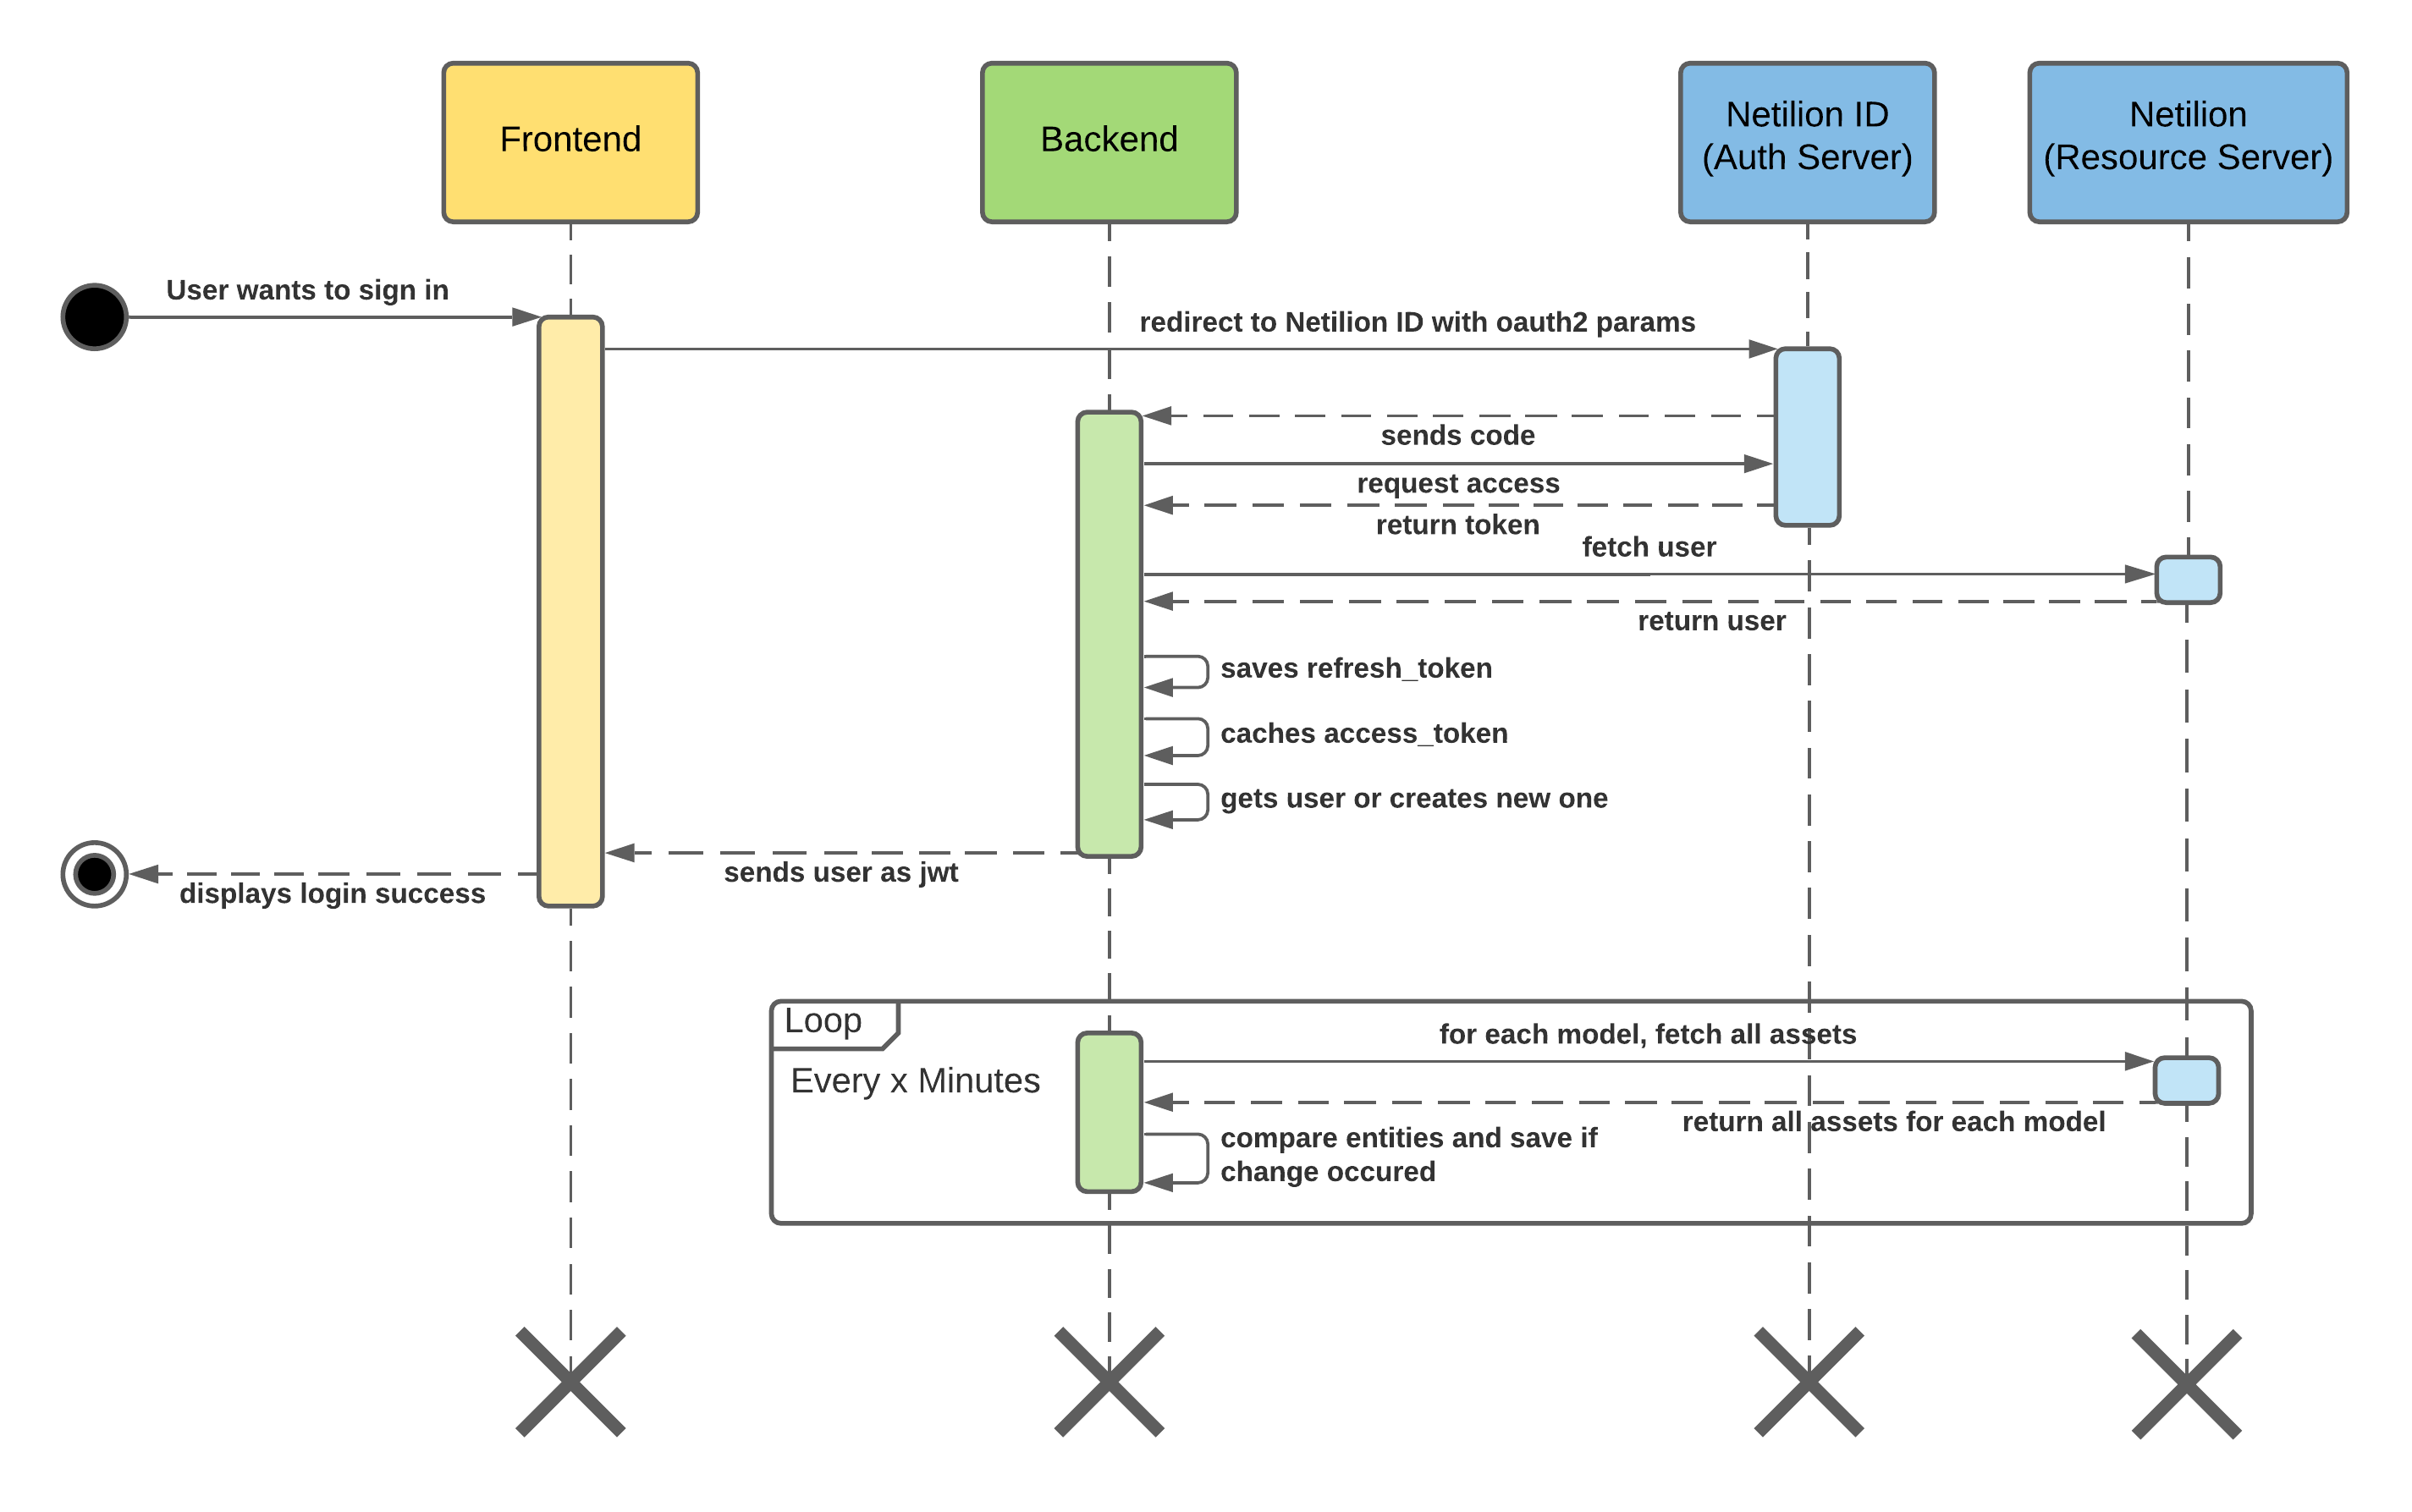
\includegraphics[width=.95\linewidth]{./images/datafetching.png}
  \caption[{Sequenzdiagram, welches das automatische fetching Erklärt}]{Data fetching in Intervallen}
  \label{fig:data-fetching}
\end{figure}
Nachdem sich ein OSE Verantwortlicher das erste mal eingeloggt hat, wird der \code{access\_token} in Redis gecached und der \code{refresh\_token} in der Datenbank gespeichert. Die Funktion soll entweder den gecachten Token nehmen und direkt zurückgeben oder mit dem \code{refresh\_token} einen neuen Anfordern, welcher wiederum gecached und zurückgegeben werden soll. Damit ist es dann möglich, dass das Backend selbst die Daten auffrischen kann. Dafür werde ich das Task-Scheduling\cite{a2021_documentation} feature von Nestjs verwenden. Damit ist es möglich eine Funktion wiederholt laufen zu lassen.
\newline
Bevor ich allerdings das ganze automatisieren kann, brauche ich eine Helferfunktion. Denn jede Anfrage an Netilion braucht einen validen \code{access\_token} und er muss auch dem Netilion Benutzer gehören, unter welchem die Messgeräte registriert sind. Mit dieser Function wird es möglich sein das ganze zu vollautomatisieren. Wenn nun ein Benutzer des OSE-Dashboards sich die Daten nun ansehen möchte, kann er dies machen, ohne den Login des jeweiligen OSE Verantwortlichen wissen zu müssen.
\pagebreak
\subsection{Zugriffskontrolle}
\subsubsection{OSE Verantwortlicher}
\begin{figure}[H]
  \centering
  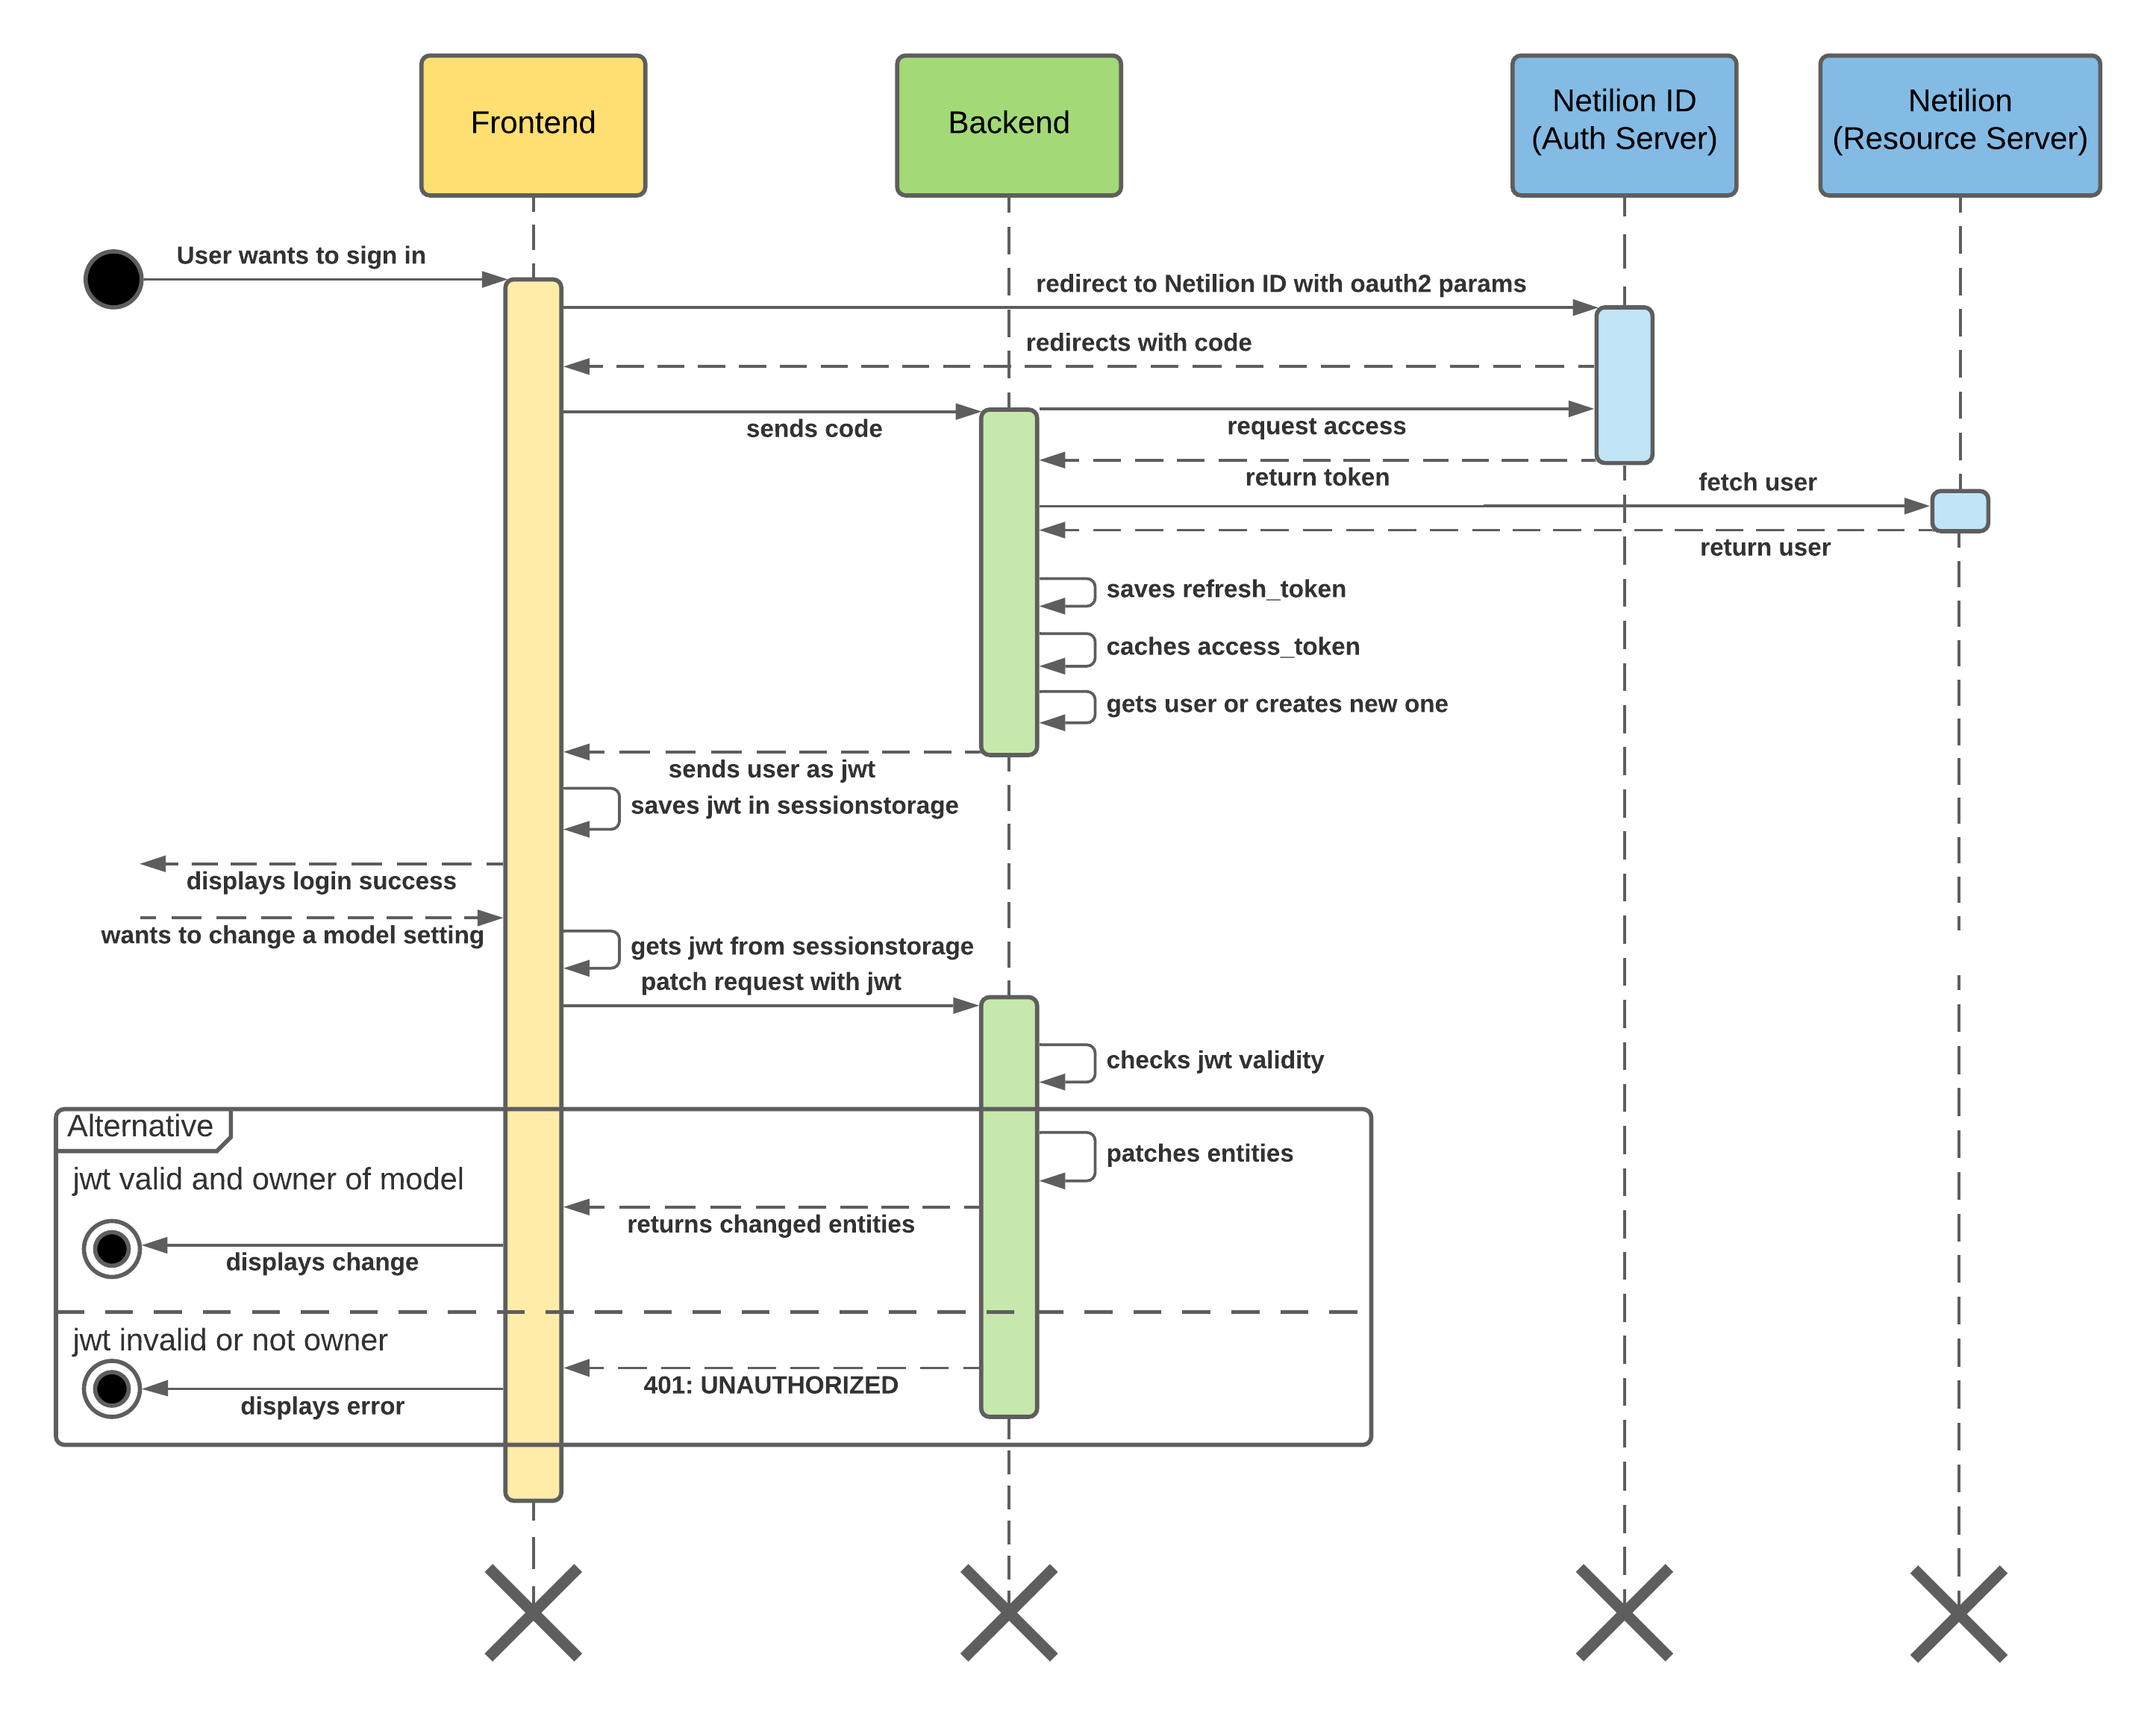
\includegraphics[width=.95\linewidth]{./images/zugriffskontrolle.png}
  \caption[{Sequenzdiagram, welches die Zugriffskontrolle für den OSE Verantwortlichen beschreibt}]{Zugriffskontrolle OSE Verantwortlicher}
  \label{fig:zugriffskontrolle}
\end{figure}
Ein OSE Verantwortlicher soll das Konfigurationsmenü seines Models öffnen können. Verantwortlicher anderer Modelle oder normale User sollen dies nicht können.
Das ganze sollte folgenderweise gelöst werden:
\newline
Das Frontend erhält nach dem erfolgreichen Login einen JWT. Dieser wird zuerst benötigt, um den Link zum Konfigurationsmenü überhaupt erst im Frontend anzuzeigen. Ausserdem wird er als Authentifizierungsmethode zum Backend verwendet. Der REST Endpoint vom Backend wird durch eine Nestjs Guard\cite{nest_guards} geschützt. Daraufhin wird direkt geprüft werden, ob das Model auch wirklich dem User gehört. Sollte dies nicht der Fall sein, wird die Anfrage als unauthorized zurückgeschickt.
\subsubsection{OSE-Dashboard Nutzer}
\begin{figure}[H]
  \centering
  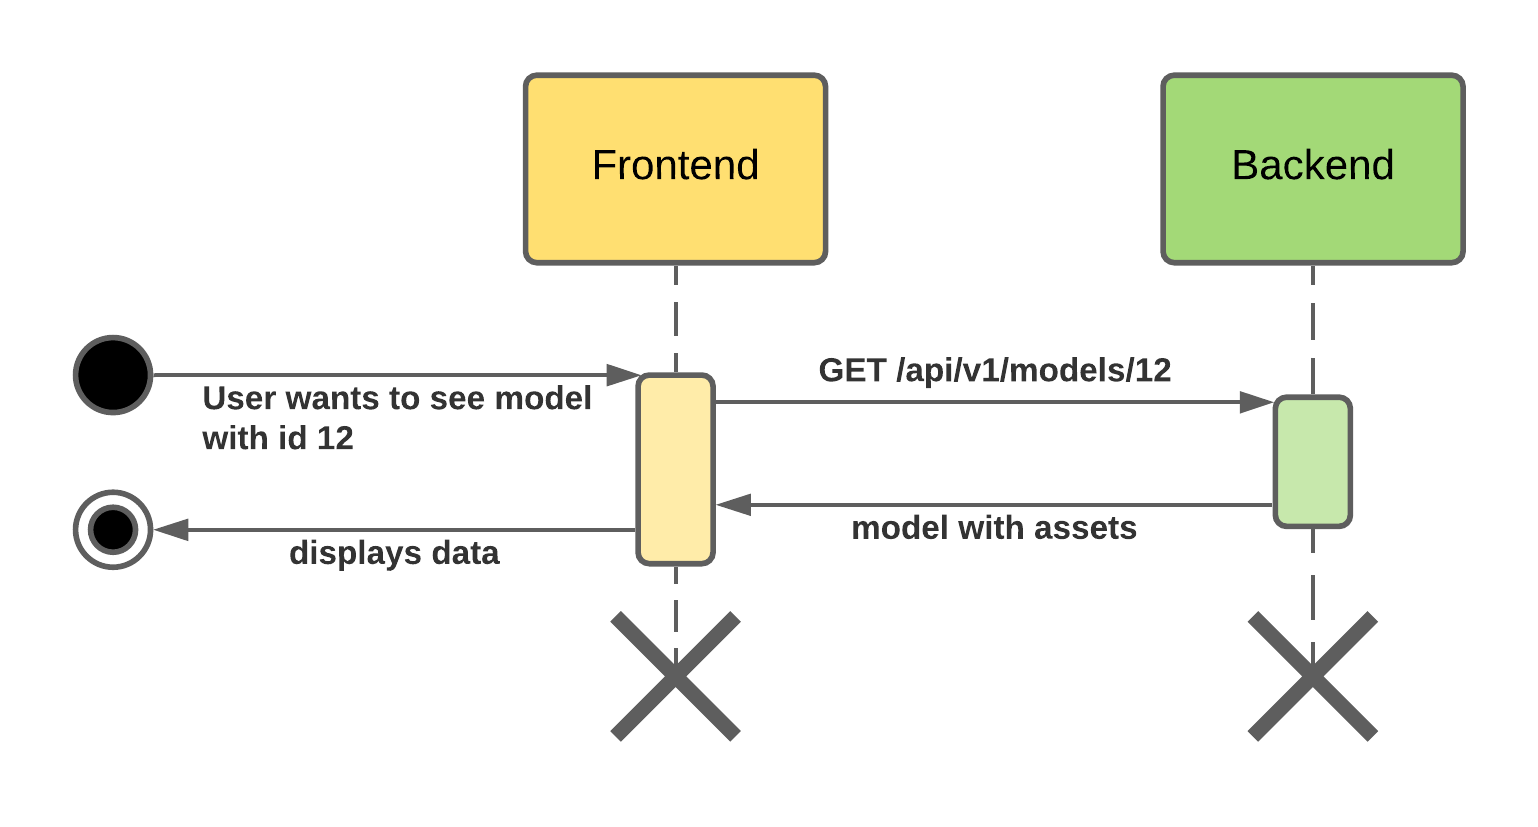
\includegraphics[width=.6\linewidth]{./images/zugriffskontrolle2.png}
  \caption[{Sequenzdiagram, welches die Zugriffskontrolle für den OSE-Dashboard Nutzer beschreibt}]{Zugriffskontrolle OSE-Dashboard Nutzer}
  \label{fig:zugriffskontrolle2}
\end{figure}
Der OSE-Dashboard möchte sich alle OSE-Modelle ansehen können, ohne sich dabei einloggen zu müssen.
Das ganze sollte folgenderweise gelöst werden:
\newline
Wie in Kapitel \ref{data-fetching} angesprochen, sind die aktuellen Daten im Backend verfügbar. So ist es also gar nicht nötig Netilion direkt anzufragen. Das Backend soll stattdessen die Daten mit einem public Endpoint verfügbar machen. Auf diesem Weg umgehen wir auch die maximale Anfragen an Netilion, welche in Kapitel \ref{arch-backend} beschrieben wurde.
\newline
So kann das Frontend beliebig oft die Daten abfragen, ohne das sich ein User einloggen muss oder das wir die Grenze der Connect Subscription übertreten.